%to do
\section{evaluation}
\label{sec:evaluation}

\begin{figure}
\centering
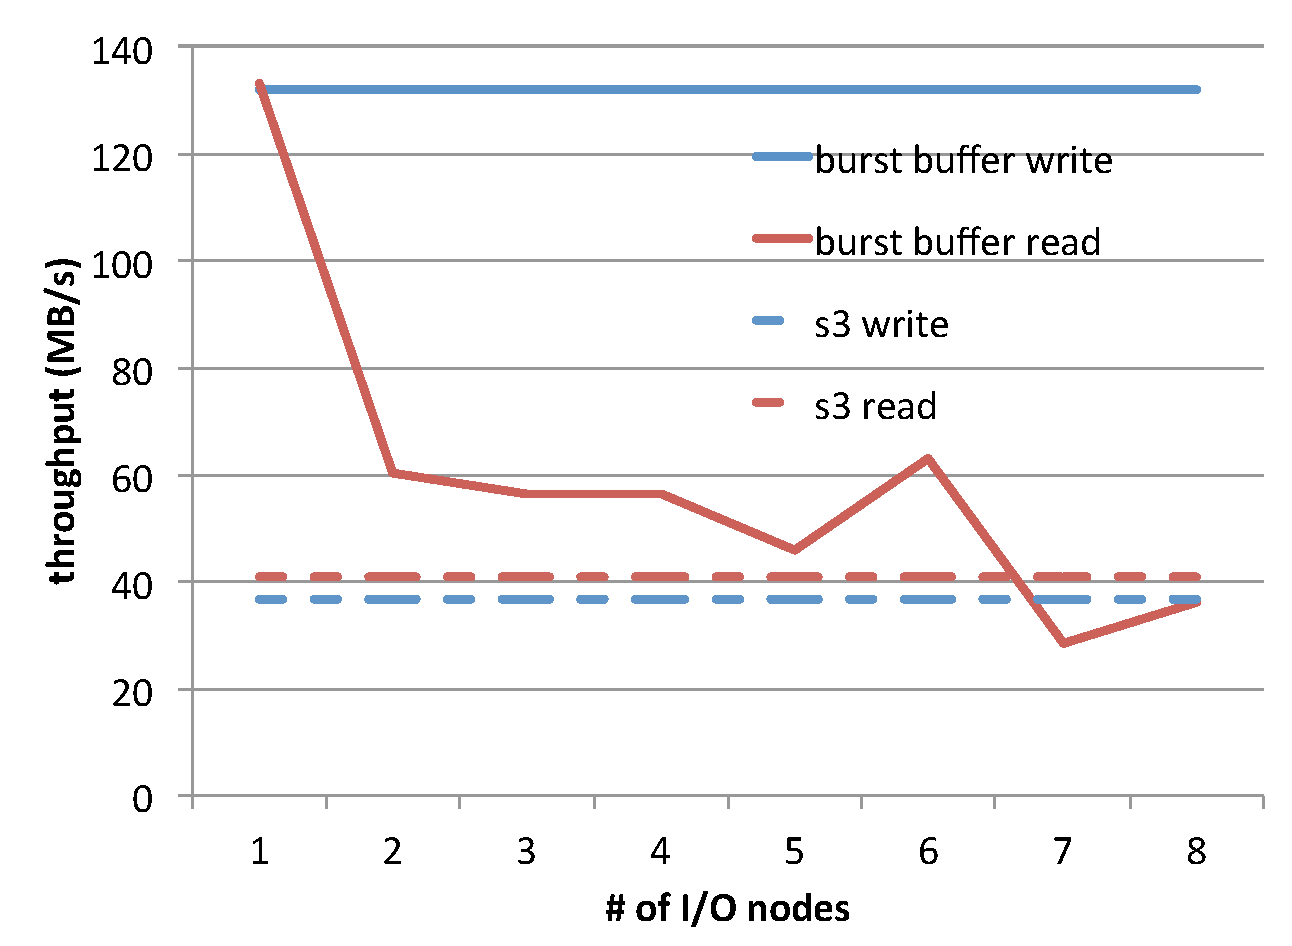
\includegraphics[width=8.5cm]{img/one_client.pdf}
\caption{One User Performance}
\label{evaluation:one user}
\end{figure}

\begin{figure}
\centering
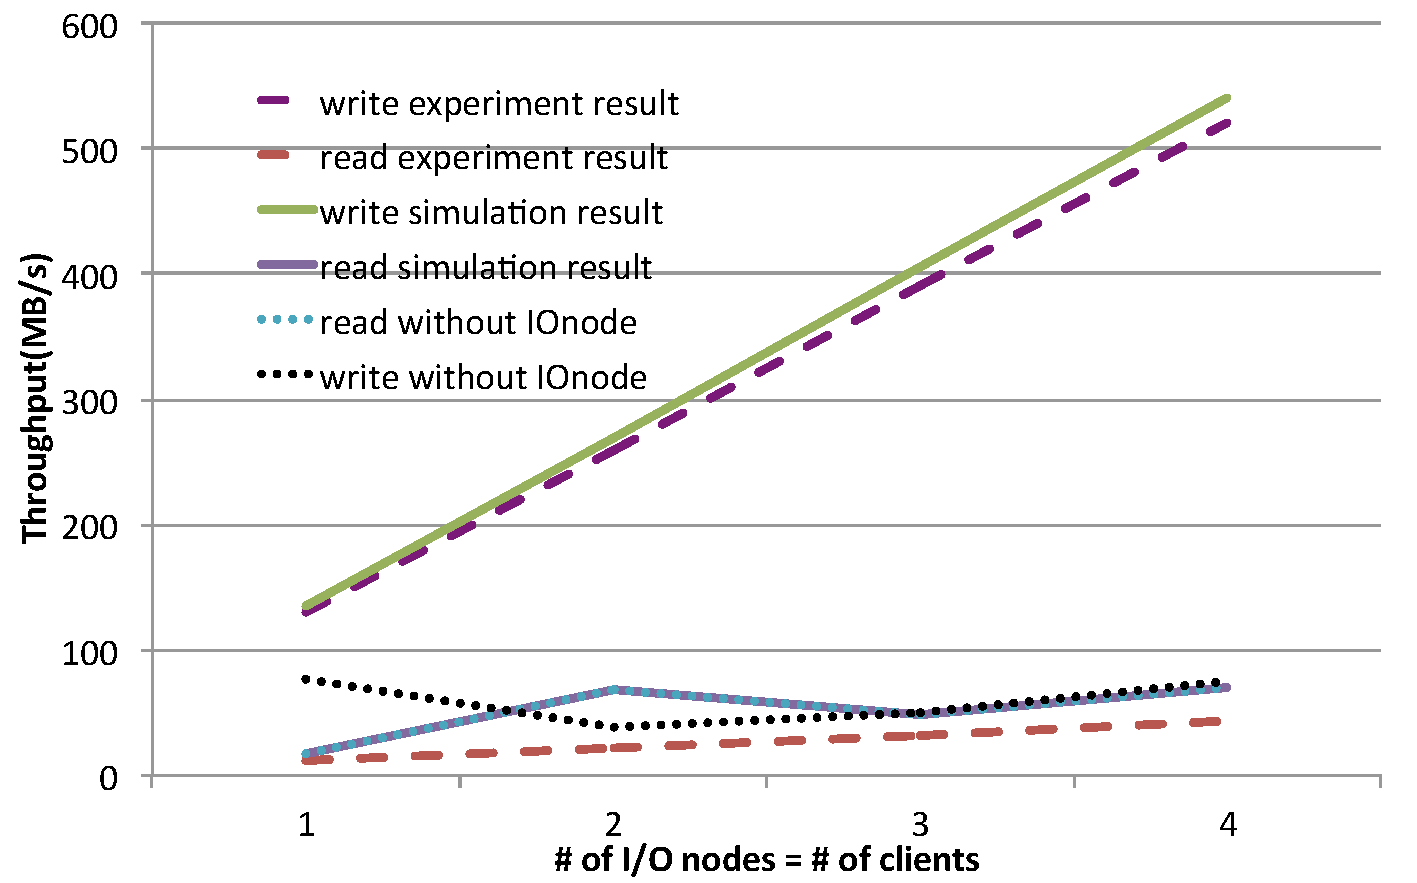
\includegraphics[width=8cm]{img/multiple_client.pdf}
\caption{Multiple User Performance}
\label{evaluation:multi user}
\end{figure}

In this section we introduce the evaluation result of our prototype implementation in Amazon EC2 public cloud.
The cloud environment is shown as Table.\ref{evaluation:amazon_environment}
\begin{table}[h]
\centering
\begin{tabular}{|c|c|}
Region				&		Tokyo		\\
Instance Type		&		m3.xlarge	\\
vCPUs				&		4			\\
ECUs				&		13			\\
Memory				&		15GiB		\\
Instance Storage	&		2*40GB(SSD)	\\
Network Performance	&		High		\\
\end{tabular}
\caption{evaluation environment}
\label{evaluation:amazon_environment}
\end{table}

\begin{table}[th]
\centering
\begin{tabular}{|c|p{150pt}|}
CPU					&		Intel\textregisted Core\texttrademark i7-3770K CPU @ 3.50GHz\\
Memory				&		16GB\\
Storage				&		

\end{tabular}
\end{table}

here vCPUs means the number of virtual CPU in instance, and one ECU provides the equivalent CPU capacity of a 1.0-1.2GHz 2007 Opteron or 2007 Xeon processor.

For the storage system, we used a machine inside our lab, the details is shows in
Table.~\ref{evaluation:stroage_environment}.

All the compute nodes, I/O nodes and master node connect with interconnection network inside Amazon
EC2, and mount storage system by sshfs\cite{sshfs} via Internet.

\subsection{One User Performance}
First we measure the performance of our prototype for only one user, and shows how our system
will affect one user performance.
In this experiment, the number of client is fixed to one, and measure
the sequential read and write performance for different number of I/O nodes.
All I/O data are distributed among all I/O nodes.
Figure~.\ref{evaluation:one user} shows one user performance.
As we know, one thread I/O is difficult to achieve the full throughput on Internet, we can see from
Figure.~\ref{evaluation:amazon_environment}

\subsection{Multiple Users Performance}
Our architecture can burst I/O performance for multiple users
X: number of client=number of I/O nodes Y:throughput

\subsection{Simulation for Applications}
Show our architecture can burst I/O performance for applications
x